%%%%%%%%%%%%%%%%%%%%%%%%%%%%%%%%%%%%%%%%%%%%%%%%%%%%%%%%%%%%%%%%%%%%%%%%%%%%%%%%%%%%%%%%%%%%%
%%									Chapitre 4												%
%%%%%%%%%%%%%%%%%%%%%%%%%%%%%%%%%%%%%%%%%%%%%%%%%%%%%%%%%%%%%%%%%%%%%%%%%%%%%%%%%%%%%%%%%%%%%

\chapter{A polynomial expansion to approximate ruin probability in the compound Poisson ruin model}\label{Chapter4}
	\minitoc
	\newpage

%%%%%%%%%%%%%%%%%%%%%%%%%%%%%%%%%%%%%%%%%%%%%%%%%%%%%%%%%%%%%%%%%%%%%%%%%%%%%%%%%%%%%%%%%%%%%



\begin{center}
\Large{\underline{\textbf{Abstract}}}\\
\end{center}
A numerical method to approximate ruin probabilities is proposed within the frame of a compound Poisson ruin model. The defective density function associated to the ruin probability is projected in an orthogonal polynomial system. These polynomials are orthogonal with respect to a probability measure that belongs to Natural Exponential Family with Quadratic Variance Function (NEF-QVF). The method is convenient in at least four ways. Firstly, it leads to a simple analytical expression of the ultimate ruin probability. Secondly, the implementation does not require strong computer skills. Thirdly, our approximation method does not necessitate any preliminary discretisation step of the claim sizes distribution. Finally, the coefficients of our formula do not depend on initial reserves. \\
%This last fact will be illustrated in the numerical illustrations conducted at the end of the paper.\\
\\
\textit{Keywords:} compound Poisson model, ultimate ruin probability, natural exponential families with quadratic variance functions, orthogonal polynomials, gamma series expansion, Laplace transform inversion.
\section{Introduction}
A non-life insurance company is assumed to be able to follow the financial reserves\rq{} evolution associated with one of its portfolios in continuous time. The number of claims until time $t$ is assumed to be an homogeneous Poisson process $\{N_{t}\}_{t\geq0}$, with intensity $\lambda$. The successive claim amounts $(U_{i})_{i\in\mathbb{N}^{*}}$, form a sequence of positive, \textbf{i.i.d.}, continuous random variables, and independent of $\{N_{t}\}_{t\geq0}$, with density function $f_{U}$ and mean $\mu$. The initial reserves are of amounts $u\geq0$, and the premium rate is constant and equal to $p\geq0$. The risk reserve process is therefore defined as 
\[
R_{t}=u+pt-\sum_{i=1}^{N_{t}}U_{i}. 
\]
The associated claims surplus process is defined as $S_{t}=u-R_{t}$. In this work, we focus on the evaluation of ultimate ruin probabilities (or infinite-time ruin probabilities) defined as 
\begin{equation}\label{UltimateRuinProba}
\psi(u)=P\left(\inf_{t\geq0}R_{t}<0|R_{0}=u\right)=P\left(\sup_{t\geq0}S_{t}>u|S_{0}=0\right).
\end{equation}
This model is called a compound Poisson model (also known as Cramer-Lundberg ruin model) and has been widely studied in the risk theory literature. See, for example, \citet{RoScScTe99,AsAl10}. We assume that the positive net profit condition holds for this model, namely $p>\lambda\mu$.\\
A useful technique in applied mathematics consists of determining a probability density function from the knowledge of its Laplace transform. We give here a brief review of the literature involving numerical inversion of Laplace transform and ruin probability approximations. In a few particular cases, the inversion of the Laplace transform associated with ruin probabilities is manageable analytically and leads to closed formula. But in most cases numerical methods are needed. The Laguerre method is an old established method based on the Tricomi-Widder Theorem of 1935. The recovered function takes the form of a sum of Laguerre functions derived through orthogonal projections. The numerical inversion of Laplace transform using Laguerre series has been originally described in \citet{We66} and improved in \citet{AbChWh95}. In the wake of Laguerre series method, we found attempts in the actuarial science literature to write probability density functions as sum of gamma densities. For instance the early work of Bowers \citet{Bo66} that  gave rise to the so-called Beekman-Bowers approximation for the ultimate ruin probability, derived in \citet{Be69}. The idea is to approximate the ultimate ruin probability by the survival function of a gamma distribution using moments fitting. Gamma series expansion has been employed  in \citet{Ta78} and later in \citet{AlTeTi01}. The authors highlight that it is useful to carry out both analytical calculations and numerical approximations. They show that the direct injection of the gamma series expression into integro-differential equations leads to reccurence relations between the expansion\rq{}s coefficients and therefore characterize them. They focus on the finite-time ruin probability but the results are valid in the infinite-time case by letting the time $t$ tend to infinity. We also want to mention the Picard-Lefevre formula, see \citet{PiLe97,RuLo04}, in which ruin probabilities are computed using the orthogonality property of the generalized Appell polynomials, defined in \citet{Po01} for instance. We explain later that our method, within the frame of ruin probabilities approximation, is closely related to the Laguerre method and represents in fact an improvement.\\

The numerical inversion via Fourier-series techniques received a great deal of interest. These techniques have been presented for instance in \citet{AbWh92} within a queueing theory setting. For an application within an actuarial framework, we refer to \citet{EmGrPi93} and \citet{RoScScTe99}, Chapter 5, Section 5.5. There is also a great body of literature dealing with Laplace transform inversion linked to the Hausdorff moment problem. Probability density function are recovered from different kind of moments. The use of exponential moments and scaled Laplace transform is presented in \citet{MnSa13} and has been performed for ruin probabilities computations in \citet{MnSaHa14}. In the work of Gzyl et al \citet{GzNITa13}, the maximum entropy applied to fractional exponential moments is employed to determine the probability of ultimate ruin. Recently, Albrecher et al. \citet{AlAvKo10} and Avram et al. \citet{AvChHo11} discuss different methods for computing the inverse Laplace transform. The first one consider a numerical inversion procedure based on a quadrature rule that uses as stepping stone a rational approximation of the exponential function in the complex plane. The second one implements and reviews much of the work done using Padé approximants to invert Laplace transform. \\

There are several usual techniques for calculation of ultimate ruin probabilities. We want to mention a classical iterative method that we will use for comparison purposes. The so-called Panjer\rq{}s algorithm introduced in \citet{Pa81}, has been widely used in the actuarial field. One can find an application to the computation of the probability of ultimate ruin in \citet{Di95}.\\

The method that we propose here consists in an orthogonal projection of the defective probability density function, associated with the probability of ultimate ruin, with respect to a reference probability measure that belongs to the Natural Exponential Families with Quadratic Variance Function. The desired defective PDF takes the form of an infinite serie of orthonormal polynomials (orthogonal with respect to the aforementioned reference probability measure). The coefficients of the expansion are defined by a scalar product and are computed from the Laplace transform or equivalently from the moments of the distribution. Ruin probability approximations are obtained through truncation of the infinite serie followed by integration. This method permits the recovery of functions from the knowledge of their Laplace transform. Once the set of coefficients of the expansion has been evaluated, ultimate ruin probabilities can be approximated for any initial reserve. It is easy to implement, does no necessitate large computation time and is competitive in terms of accuracy.  The approximation of the ruin probability allows manipulations such as integration or reinjection in formulas to derive approximations of distributions that governed other quantities of interest in ruin theory. For instance, the probability density function of the surplus prior to ruin involves the ultimate ruin probability, we refer to \citet{Di92,GeSh98} for more details.\\

This work is also a theoretical background in view of a future statistical application. Many papers deals with statistical estimation of ruin probabilities when observations of the claim sizes are available. The use of a Laplace inversion formula as basis for a nonparametric estimator has already been employed for ruin probabilities estimation in \citet{MnRuRu08,ZhYaYa14}, scaled Laplace transform and the maximum of entropy may offer the same possibility and would be based on empirical estimation of the moments. The definition of the coefficients in our method are based on quantities that are well adapted to empirical estimations. By plugging in the estimators of the coefficients, we will obtain a nonparametric estimator taking the form of an orthogonal serie. The investigation of ruin probability statistical estimation will be at the center of a forthcomiong paper, for now we only consider ruin probability approximations.\\

In Section 2, we introduce a density expansion formula based on orthogonal projection within the frame of NEF-QVF. Our main results are developed in Section 3: the expansion for ultimate ruin probabilities is derived, a sufficient condition of applicability is given and the goodness of the approximation is discussed. Section 4 is devoted to numerical illustrations. Just like what is done in \citet{GzNITa13},  we compare our method to other existing methods, namely Panjer's algorithm, Fast Fourrier Transform and scaled Laplace transform inversion.
\section{Polynomial expansions of a probability density function}
Let $F=\{F_{\theta},\theta\in\Theta\}$ with $\Theta\subset \mathbb{R}$ be a Natural Exponential Family (NEF), see \citet{Ba78}, generated by a probability measure $\nu$ on $\mathbb{R}$ such that
\begin{eqnarray*}
F_{\theta}(X\in A)&=&\int_{A}exp\{x\theta-\kappa(\theta)\}\text{d}\nu(x)\\
&=&\int_{A}f(x,\theta)\text{d}\nu(x),
\end{eqnarray*}
where $A\subset\mathbb{R}$, $\kappa(\theta)=log\left(\int_{\mathbb{R}}e^{\theta x}\text{d}\nu(x)\right)$ is the Cumulant Generating Function (CGF) and $f(x,\theta)$ is the density of $F_{\theta}$ with respect to $\nu$.
Let $X$ be a random variable  $F_{\theta}$-distributed. The mean of the random variable $X$, is given by
\begin{equation*}
m=E_{\theta}(X)=\int x\text{d}F_{\theta}(x)=\kappa'(\theta),
\end{equation*}
and its variance is
\begin{equation}
V(m)=Var_{\theta}(X)=\int (x-m)^{2}\text{d}F_{\theta}(x)=\kappa''(\theta).\label{Variance}
\end{equation}
The application $\theta\rightarrow\kappa'(\theta)$ is one to one. Its inverse function $m\rightarrow h(m)$ is defined on $\cal{M}$ $=\kappa'(\Theta)$. With a slight change of notation, we can rewrite $F=\{F_{m},m \in\cal{M}\}$, where $F_{m}$ has mean $m$ and density $f(x,m)=exp\{h(m)x-\kappa(h(m))\}$ with respect to $\nu$. A NEF has a Quadratic Variance Function (QVF) if there exists reals $v_0, v_1, v_2$ such that 
\begin{equation}\label{QVF}
V(m)=v_{0}+v_{1}m+v_{2}m^{2}.
\end{equation}
The Natural Exponential Families with Quadratic Variance Function (NEF-QVF) include the normal, gamma, hyperbolic, Poisson, binomial and negative binomial distributions.\\
Define
\begin{equation}\label{Poly1}
P_{n}(x,m)=V^{n}(m)\left\{\frac{\partial^{n}}{\partial m^{n}}f(x,m)\right\}/f(x,m),
\end{equation}
for $n\in\mathbb{N}$. Each $P_{n}(x,m)$ is a polynomial of degree $n$ in both $m$ and $x$. Moreover, if $\nu$ is a NEF-QVF, $(P_{n})_{n\in\mathbb{N}}$ is a family of orthogonal polynomials with respect to $\nu$ in the sense that
\[
<P_{n},P_{m}>=\int P_{n}(x,m)P_{m}(x,m)f(x,m)\text{d}\nu(x)=\delta_{nm}||P_{n}||^{2},\hspace{1cm}m,n\in\mathbb{N},
\]
where $\delta_{mn}$ is the Kronecker symbol equal to $1$ if $n=m$ and $0$ otherwise. For the sake of simplicity, we choose $\nu=P_{m_{0}}$. Then $f(x,m_{0})=1$ and we write
\begin{equation}\label{Poly2}
P_{n}(x)=P_{n}(x,m_{0})=V^{n}(m_{0})\left\{\frac{\partial^{n}}{\partial m^{n}}f(x,m)\right\}_{m=m_{0}}.
\end{equation}
We also consider in the rest of the paper a normalized version of the polynomials defined in \eqref{Poly2} with $Q_{n}(x)=P_{n}(x)/||P_{n}||$. For an exhaustive review regarding NEF-QVF and their properties, we refer to \citet{Mo82}.\\
We denote by $L^{2}(\nu)$ the space of functions square integrable with respect to $\nu$.
\begin{Prop}\label{PolyExpansiontheo}
Let $\nu$ be a probability measure that generates a NEF-QVF, with associated orthonormal polynomials $\{Q_n\} _{n\in\mathbb{N}}$. Let $X$ be a random variable with density function $\frac{dP_{X}}{\text{d}\nu}$  with respect to $\nu$. If $\frac{\text{d}F_{X}}{\text{d}\nu}\in L^{2}(\nu)$ then we have the following expansion
\begin{eqnarray}
\frac{\text{d}F_{X}}{\text{d}\nu}(x)%&=&\sum^{+\infty}_{n=0}<\frac{P_{n}}{||P_{n}||},\frac{dP_{X}}{dP_{0}}>Q_{n}(x),\label{PolyExpansionEqnl1}\\
&=&\sum^{+\infty}_{n=0}E(Q_{n}(X))Q_{n}(x). \label{PolyExpansionEqnl3}
\end{eqnarray}
\end{Prop}
\begin{proof}
%We know that $\{P_{n}\}_{n\in\mathbb{N}}$ is an orthogonal polynomials system with respect to  $P_{0}$. As polynomials are dense in $L^{2}(P_{0})$,   
By construction $\{Q_{n}\}_{n\in\mathbb{N}}$ forms an orthonormal basis of $L^{2}(\nu)$, 
%the first equality \eqref{PolyExpansionEqnl1} is obtained though 
and by orthogonal projection we get
%, and the last one \eqref{PolyExpansionEqnl3} follows from
\begin{eqnarray*}
\frac{\text{d}F_{X}}{\text{d}\nu}(x)&=&\sum^{+\infty}_{n=0}<Q_{n},\frac{\text{d}F_{X}}{\text{d}\nu}>Q_{n}(x).
%\label{PolyExpansionEqnl1}\\
%&=&\sum^{+\infty}_{n=0}E(P_{n}(X))Q_{n}(x). \label{PolyExpansionEqnl3}
\end{eqnarray*}
It follows that 
\begin{eqnarray*}
<Q_n,\frac{\text{d}F_{X}}{\text{d}\nu}>Q_{n}(x)&=&\int Q_{n}(y)\frac{\text{d}F_{X}}{\text{d}\nu}(y)\text{d}\nu(y)\times Q_{n}(x)\\
&=&\int Q_{n}(y)\text{d}F_{X}(y)\times Q_{n}(x) \\
&=&E(Q_{n}(X))Q_{n}(x).
\end{eqnarray*}
\end{proof}
Denote by $f_{\nu}$ and $f_{X}$ the probability density functions of $\nu$ and $X$ respectively. Proposition \ref{PolyExpansiontheo} gives an expansion of $f_{X}$ that takes the following simple form
\begin{equation}\label{PDFPolynomialExpansion}
f_{X}(x)=\sum^{+\infty}_{n=0}a_{n}Q_{n}(x)f_{\nu}(x),
\end{equation} 
where $(a_{n})_{n\in\mathbb{N}}$ is a sequence of real number called coefficients of the expansion in the rest of the paper, $(Q_{n})_{n\in\mathbb{N}}$ is an orthonormal sequence of polynomials with respect to $\nu$, and $f_{\nu}$ is the PDF of $\nu$. The polynomials $(Q_{n})_{n\in\mathbb{N}}$ are of degree $n$ in $x$ and can therefore be written as $Q_{n}(x)=\sum^{n}_{i=0} q_{i,n}x^{i}$. Using this last remark, we rewrite the coefficients of the expansion as 
\begin{eqnarray}
a_{n}&=&E(Q_{n}(X))\nonumber\\
&=&\sum_{i=1}^{n}q_{i,n}E\left(X^{i}\right)\label{CoefStatistical}\\
&=&\sum_{i=1}^{n}q_{i,n}(-1)^{i}\left[\frac{d^{i}\widehat{f_{X}}(s)}{ds^{i}}\right]_{s=0}\nonumber,
\end{eqnarray} 
where $\widehat{f_{X}}(s)=\int e^{-sx}\text{d}F_{X}(x)$ is the Laplace transform of the random variable $X$. The approximation of the PDF of $X$ is obtained by truncation of the infinite serie in \eqref{PDFPolynomialExpansion}. First, we choose a NEF-QVF, then we choose a member of this family characterized by its parameters. These choices are to be made wisely so as to ensure the validity of the expansion and to reach an acceptable level of accuracy that goes along with an order of truncation as small as possible. In the light of the expression of the coefficients \eqref{CoefStatistical}, it seems natural to consider a statistical extension that would lead to a nonparametric estimator of the probability density function. However, it is of interest to start with the probabilistic problem as it is the theoretical basis for a statistical application. The next section shows how to use the orthogonal polynomials and NEF-QVF framework to approximate ruin probabilities. 
\section{Application to the ruin problem}
\subsection{General formula}
The ultimate ruin probability in the compound Poisson ruin model is the survival function of a geometric compound distributed random variable
\begin{equation}\label{RandomVariableGeometricCompound}
M=\sum^{N}_{i=1}U_{i}^{I},
\end{equation}
where $N$ is a counting random variable having a geometric distribution with parameter $\rho=\frac{\lambda\mu}{p}$, and $(U^{I}_{i})_{i\in\mathbb{N}^{*}}$ is a sequence of independent and identically distributed nonnegative random variables having PDF defined as $f_{U^{I}}(x)=\frac{\overline{F_{U}}(x)}{\mu}$. The distribution of $M$ has an atom at $0$ with probability mass $P(N=0)=1-\rho$. The probability measure that governs $M$ is
\begin{equation}
\text{d}F_{M}(x)=\left(1-\rho\right)\delta_{0}(x)+\text{d}G_{M}(x),
\end{equation}
where $\text{d}G_{M}$ is the continuous part of the probability measure associated to $M$ which admits a defective probability density function with respect to the Lebesgue measure. We denote by $g_{M}$ the defective probability density function. The ultimate ruin probability follows from the integration of the the continuous part as the discrete part vanishes 
\begin{eqnarray*}
\psi(u)=P(M>u)=\int_{u}^{+\infty}\text{d}G_{M}(x).
\end{eqnarray*}
\begin{Theo}\label{RuinProbabilityExpansionTheo}
Let $\nu$ be an univariate distribution having a probability density function with respect to the Lebesgue measure that generates a NEF-QVF. Let $(Q_{n})_{n\in\mathbb{N}}$ be the sequence of orthonormal polynomials with respect to $\nu$. If $\frac{\text{d}G_{M}}{\text{d}\nu}\in L^{2}(\nu)$ then
\begin{equation}\label{RuinProbabilityExpansion}
\psi(u)=\sum^{+\infty}_{n=0}a_{n}\int^{+\infty}_{u}Q_{n}(x)\text{d}\nu(x),
\end{equation}
where $(a_{n})_{n\in\mathbb{N}}$ is defined as in \eqref{CoefStatistical}. 
\end{Theo}
\begin{proof}
We apply Proposition \ref{PolyExpansiontheo} to get the result.
\end{proof}
\subsection{Approximation with Laguerre polynomials}
We derive an approximation for the ultimate ruin probability, using Theorem \ref{RuinProbabilityExpansionTheo}, combined with truncations of order $K$ of the infinite series in \eqref{RuinProbabilityExpansion}. It yields
\begin{equation}\label{RuinProbabilityApproximation}
\psi_{K}(u)=\sum_{n=0}^{K}a_{n}\int^{+\infty}_{u}Q_{n}(x)\text{d}\nu(x),
\end{equation}
the approximated ruin probability with order of truncation $K$.
As the distribution of $M$ has support on $\mathbb{R}^{+}$, we choose the Gamma distribution $\Gamma(r,m)$ with mean parameter $m$ and shape parameter $r$, that is:
\[
\text{d}\nu(x)=f_{\nu}(x)\bold{1}_{\mathbb{R}^{+}}(x)d\lambda(x)=\frac{x^{r-1} e^{-x/m}}{\Gamma(r)m^{r}}\bold{1}_{\mathbb{R}^{+}}(x)d\lambda(x).
\]
The associated orthogonal polynomials are the generalized Laguerre polynomials. By definition, they satisfy the following orthogonality condition
\[
\int_{0}^{+\infty}L^{r-1}_{n}(x)L^{r-1}_{m}(x)x^{r-1}e^{-x}dx=\binom{n+r-1}{n}\Gamma(r)\delta_{nm}.
\]
The polynomials involved in the ruin probability approximation in \eqref{RuinProbabilityApproximation} are the generalized Laguerre polynomials with a slight change in comparison to the definition given in \citet{Sz39}, namely
\begin{equation}
Q_{n}(x)=(-1)^{n}\binom{n+r-1}{n}^{-1/2}L^{r-1}_{n}(x/m).
\end{equation}
\begin{Rk}\label{RkLaguerreMethod}
The Laguerre functions are defined in \citet{AbChWh95} as 
\begin{equation}\label{LaguerreFunction}
l_{n}(x)=e^{-x/2}L_{n}(x),\hspace{0.1cm}x\geq0.
\end{equation}
The application of the Laguerre method consists in representing $g_{M}$ as a Laguerre serie
\begin{equation}\label{LaguerreSerieRepresentation}
g_{M}(x)=\sum_{n=0}^{+\infty}a_{n}l_{n}(x).
\end{equation} 
The representation \eqref{LaguerreSerieRepresentation} is close to the proposed expansion when choosing $r=1$ and $m=2$ as pararmeter of the reference measure. The difference lies in the possibility of changing the parameters in our expansion. We will see later that the parametrization is of prime importance. 
\end{Rk}
The defective probability density function associated to $G_{M}$ has the following expression
\begin{equation}\label{DefectiveDensityFunction}
g_{M}(x)=\sum^{+\infty}_{n=1}(1-\rho)\rho^{n}f^{*n}_{U^{I}}(x).
\end{equation}
Taking the Laplace transform of the defective probability density function defined as in \eqref{DefectiveDensityFunction} yields
\begin{equation}\label{LaplaceTransform}
\widehat{g_{M}}(s)=\frac{(1-\rho)\rho\widehat{f_{U^{I}}}(s)}{1-\rho\widehat{f_{U^{I}}}(s)},
\end{equation}
where $\widehat{f_{U^{I}}}(s)=\int e^{-sx}f_{U^{I}}(x)dx$ is the Laplace transform of $f_{U^{I}}$. The Laplace transform of the claim size distribution appears in the formula. This fact limits the application to claim sizes distributions that admit a well defined Laplace transform, namely light-tailed distributions. We want to mention that this problem might be reconsidered once the study of the statistical extension will be done. In \citet{MnSaHa14}, approximations of the ruin probability in case of heavy tail claim amounts are derived from the associated nonparametric estimator computed with simulated data.
\subsection{Integrability condition}
We illustrate here how the applicability of the method is subject to the parametrization, namely the choice of $m$ and $r$. The parametrization permits to ensure the integrability condition. The adjustment coefficient $\gamma$ is the unique positive solution of the so-called Cramer-Lundberg equation
\begin{equation}\label{LundbergEquation}
\widehat{m_{U^{I}}}(s)=\frac{1}{\rho},
\end{equation}
where $\widehat{m_{U^{I}}}(s)=\int_{0}^{+\infty}e^{sx}f_{U^{I}}(x)dx$ is the moment generating function of $U^{I}$. The integrability condition $\frac{\text{d}G_{M}}{\text{d}\nu}\in L^{2}(\text{d}\nu)$ is equivalent to 
\begin{equation}\label{IntegrabiltyCondition}
\int^{+\infty}_{0}g_{M}^{2}(x) e^{x/m}x^{1-r}dx<\infty.
\end{equation}
In order to ensure this condition, we need the following result.
\begin{Theo}\label{Theo3}
Assume that the Cramer-Lundberg equation \eqref{LundbergEquation} admits a positive solution $\gamma$, then for all $x\geq0$
\begin{equation}\label{InequalityDefectiveCompoundDensity}
g_{M}(x)\leq C(s_{0})e^{-s_{0} x},
\end{equation}
with $s_{0}\in[0,\gamma)$ and $C(s_{0})\geq0$.
\end{Theo}
\begin{proof}
In order to prove the theorem we need the following lemma regarding the survival function $\overline{F_{U}}$ of the claim sizes distribution.
\begin{Lemm}\label{TechnicalLemma1}
Let $U$ be a non-negative random variable. Assume that there exists $s_{0}>0$ such that $\widehat{
m_{U}}(s_{0})<+\infty$. Then there exists $A(s_{0})>0$ such that for all $x\geq 0$
\begin{equation}
\overline{F_{U}}(x)\leq A(s_{0})e^{-s_{0}x}.
\end{equation} 
\end{Lemm}
\begin{proof}
As $\widehat{m_{U}}(s_{0})<+\infty$, we have
\begin{eqnarray*}
\widehat{m_{U}}(s_{0})-1&=&\int_{0}^{+\infty}(e^{s_{0}x}-1)f_{U}(x)dx\\
&=&s_{0}\int_{0}^{+\infty}\int^{x}_{0}e^{s_{0}y}f_{U}(x)dydx\\
%&=&s_{0}\int_{0}^{+\infty}e^{s_{0}y}\int^{+\infty}_{y}f_{U}(x)dxdy\\
&=&s_{0}\int_{0}^{+\infty}e^{s_{0}y}\overline{F_{U}}(y)dy\\
&\geq&s_{0}\int_{0}^{x}e^{s_{0}y}\overline{F_{U}}(y)dy\\
&\geq&\overline{F_{U}}(x)(e^{s_{0}x}-1).
\end{eqnarray*}
thus, we deduce that $\forall x\geq0$
\begin{eqnarray}
\overline{F_{U}}(x)\leq(\widehat{m_{U}}(s_{0})-1+\overline{F_{U}}(x))e^{-s_{0}x}.
\end{eqnarray}
\end{proof}
The equation \eqref{LundbergEquation} is equivalent to 
\begin{equation}\label{LundbergEquationRemastered}
\rho\widehat{m_{U}}(s)=1+s\mu.
\end{equation}
The fact that $\gamma$ is a solution of the equation \eqref{LundbergEquation} implies that $\widehat{m_{U}}(s)<+\infty,\hspace{0,1cm} \forall s_{0}\in[0,\gamma)$ and by application of Lemma \ref{TechnicalLemma1}, we get the following inequality upon the PDF of $U^{I}$
\begin{equation}
f_{U^{I}}(x)=\frac{\overline{F_{U}}(x)}{\mu}\leq B(s_{0})e^{-s_{0}x}.
\end{equation}
In view of \eqref{DefectiveDensityFunction}, it is easily checked that $g_{M}$ satisfies the defective renewal equation
\begin{equation}\label{RenewalEquation}
g_{M}(x)=\rho(1-\rho)f_{U^{I}}(x)+\rho\int_{0}^{x}f_{U^{I}}(x-y)g_{M}(y)dy.
\end{equation}
We can therefore bound $g_{M}$ as in \eqref{InequalityDefectiveCompoundDensity}
\begin{eqnarray*}
g_{M}(x)&\leq& \rho(1-\rho)f_{U^{I}}(x)+\int_{0}^{+\infty}f_{U^{I}}(x-y)g_{M}(y)dy\\
&\leq& \rho(1-\rho)B(s_{0})e^{-s_{0}x}+B(s_{0})e^{-s_{0}x}\int_{0}^{+\infty}e^{s_{0}y}g_{M}(y)dy\\
&=&(\rho(1-\rho)+\widehat{g_{M}}(-s_{0}))B(s_{0})e^{-s_{0}x}\\
&=&C(s_{0})e^{-s_{0}x}.
\end{eqnarray*}
\end{proof}
Applying Theorem \ref{Theo3} yields a sufficient condition in order to use the polynomial expansion.
\begin{Cor}\label{CoroParam}
For $\frac{1}{m}<2\gamma$ and $r=1$, the integrability condition \eqref{IntegrabiltyCondition} is satisfied.
\end{Cor}
The choice of the parameter $m$ is important. The Laguerre method, briefly described in Remark \ref{RkLaguerreMethod}, does not offer the possibility of changing the parameter. In the next subsection, we shed light on another key aspect of parametrization. 
\subsection{On the goodness of the approximation}
The approximation is obtained through the truncation of an infinite serie. The higher the order of truncation gets, the better the approximation is. Our goal is to work out an efficient numerical method that combines high accuracy and small computation time. We want to minimize the number of coefficients to compute. The sequence of coefficients of the expansion must decrease as fast as possible. we assume that $\frac{\text{d}G_{M}}{\text{d}\nu}\in L^{2}(\nu)$ in order to apply the method and consequently
\begin{equation}\label{SquareSummability}
<\frac{\text{d}G_{M}}{\text{d}\nu},\frac{\text{d}G_{M}}{\text{d}\nu}>=\sum^{+\infty}_{n=0}a_{n}^{2}<+\infty.
\end{equation}  
%which implies that $a_{n}\arrow+\infty$ as $n\arrow +\infty$. We can also bound the coefficients, recall that
%\begin{equation}
%a_{n}=<Q_{n},\frac{\text{d}G_{M}}{\text{d}\nu}>=\int_{0}^{+\infty}Q_{n}(x)g_{M}(x)dx\nonumber.
%\end{equation}
%Then we have 
%\begin{equation}
%|a_{n}|\neq\int_{0}^{+\infty}Q_{n}(x)g_{M}(x)dx\nonumber.
%\end{equation}
The Parseval type relation \eqref{SquareSummability} implies that the coefficients of the expansion decrease towards $0$ as $n$ tends to infinity. The question is how fast is the decay? We address this problem using generating function theory, just like what is done in \citet{AbChWh95}. Taking the Laplace transform of $g_{M}$ defined as a polynomial expansion yields
\begin{eqnarray*}
\widehat{g_{M}}(s)&=&\int_{0}^{+\infty}e^{-sx}\sum_{n=0}^{+\infty}a_{n}Q_{n}(x)f_{\nu}(x)dx \nonumber\\
&=&\sum_{n=0}^{+\infty}a_{n}\int_{0}^{+\infty}e^{-sx}Q_{n}(x)f_{\nu}(x)dx.\nonumber\\
\end{eqnarray*}
The orthonormal polynomial system $(Q_{n})_{n\in\mathbb{N}}$ are Laguerre's one, defined as
\begin{equation}\label{GammaOrthonormalPolynomial}
Q_{n}(x)=\frac{(-1)^{n}}{\sqrt{\binom{n+r-1}{n}}}L^{r-1}_{n}\left(\frac{x}{m}\right),
\end{equation}
where $L^{r-1}_{n}(x)=\sum_{i=0}^{n}\binom{n+r-1}{n-i}\frac{(-x)^{i}}{i!}$. We refer to \citet{Sz39} for this last definition. We then have
\begin{eqnarray}
\widehat{g_{M}}(s)&=&\sum_{n=0}^{+\infty}a_{n} \int_{0}^{+\infty}e^{-sx}\frac{(-1)^{n}}{\sqrt{\binom{n+r-1}{n}}}L^{r-1}_{n}\left(\frac{x}{m}\right)\frac{x^{r-1}e^{-x/m}}{\Gamma(r)m^{r}}dx\nonumber\\
&=&\sum_{n=0}^{+\infty}a_{n}\frac{(-1)^{n}}{\sqrt{\binom{n+r-1}{n}}}\int^{+\infty}_{0}e^{-sx}\sum_{i=0}^{n}\binom{n+r-1}{n-i}\frac{(-x)^{i}}{i!m^{r}}\frac{x^{r-1}e^{-x/m}}{\Gamma(r)m^{r}}dx\nonumber\\
&=&\sum_{n=0}^{+\infty}a_{n}\frac{(-1)^{n}}{\sqrt{\binom{n+r-1}{n}}}\sum_{i=0}^{n}\frac{(n+r-1)!}{(n-i)!(r+i-1)!(r-1)!i!}(-1)^{i}\int^{+\infty}_{0}e^{-sx}\frac{x^{r+i-1}e^{-x/m}}{m^{r+i}}dx\nonumber\\
&=&\sum_{n=0}^{+\infty}a_{n}(-1)^{n}\sqrt{\binom{n+r-1}{n}}\sum_{i=0}^{n}\binom{n}{i}(-1)^{i}\int^{+\infty}_{0}e^{-sx}\frac{x^{r+i-1}e^{-x/m}}{m^{r+i}\Gamma(r+i)}dx\nonumber\\
&=&\sum_{n=0}^{+\infty}a_{n}(-1)^{n}\sqrt{\binom{n+r-1}{n}}\sum_{i=0}^{n}\binom{n}{i}(-1)^{i}\left(\frac{1}{sm+1}\right)^{r+i}\nonumber\\
&=&\sum_{n=0}^{+\infty}a_{n}(-1)^{n}\sqrt{\binom{n+r-1}{n}}\left(\frac{1}{sm+1}\right)^{r}\left(\frac{sm}{sm+1}\right)^{n}\nonumber\\
&=&\sum_{n=0}^{+\infty}a_{n}I_{\nu}(n)G_{\nu}(s)H_{\nu}(s)^{n}\nonumber,
\end{eqnarray}
where $I_{\nu}(n)=(-1)^{n}\sqrt{\binom{n+r-1}{n}}$, $G_{\nu}(s)=\left(\frac{1}{sm+1}\right)^{r}$ and $H_{\nu}(s)=\frac{sm}{sm+1}$. Define $b_{n}=I_{\nu}(n)a_{n}, \forall n\in \mathbb{N}$, we have
\begin{equation}
\widehat{g_{M}}(s)=G_{\nu}(s)B(H_{\nu}(s))\label{GeneratingFunctionToLaplaceTransform},
\end{equation}
where $B(z)=\sum^{+\infty}_{n=0}b_{n}z^{n}$ is the generating function of the sequence $(b_{n})_{n\in\mathbb{N}}$. The generating function $B$ is expressed as a function of the Laplace transform of $g_{M}$ via a change of variable
\begin{eqnarray}
B(z)&=&\frac{\widehat{g_{M}}(H^{-1}_{\nu}(z))}{G_{\nu}(H^{-1}_{\nu}(z))}\nonumber\\
&=&(1-z)^{-r}\widehat{g_{M}}\left(\frac{z}{m(1-z)}\right).\label{LaplaceTransformToGeneratingFunction}
\end{eqnarray}  
In generating function theory, it is possible to study the decay of a sequence by considering its radius of convergence. If the radius of convergence of $B(z)$ is greater than one then the sequence of coefficients admits a decay that is geometrically fast. Non-geometric convergence occurs when $B$ admits a singularity on the unit circle $\{z:|z|=1\}$. The parameters of the expansion permit to alter the form of the generating function in order to make it simpler. Sometimes it gets so simple that an exact formula is obtained. The two following examples may help convince the reader. 
\begin{Ex}\label{GammaPDFExpansion}
In \citet{AbChWh95}, several attempts are made to expand PDF when the convergence is not geometrically fast. One of those cases is the expansion of a Gamma PDF $\Gamma(\alpha,\beta)$, recall that the PDF is given by 
\begin{equation}
f_{X}(x)=\frac{x^{\alpha-1}e^{-x/\beta}}{\beta^{\alpha}\Gamma(\alpha)},
\end{equation}
with associated Laplace transform
\begin{equation}
\widehat{f_{X}}(s)=\left(\frac{1}{1+\beta s}\right)^{\alpha}.
\end{equation}
The generating function of the coefficient defined in \eqref{LaplaceTransformToGeneratingFunction} is
\begin{equation}
B(z)=\frac{m^{\alpha}(1-z)^{\alpha-r}}{(m-z(\beta-m))^{\alpha}}.
\end{equation} 
It is easily checked that taking $r=\alpha$ and $m=\beta$ yields $B(z)=1$. Thus we deduce that $a_{0}=1$ and $a_{n}=0,\forall n\geq1$.  
\end{Ex}
\begin{Ex}\label{UltimateRuinProbabilityExponentialCaseExample}
The exact ultimate ruin probability for the classical ruin model is available in a closed form when the claim sizes are governed by an exponential distribution $\Gamma(1,\beta)$. In this particular case, the integrated tail distribution is also an exponential distribution with the same parameter as the claim amounts. Assume that the claim sizes are $\Gamma(1,\beta)-distributed$. The Laplace transform of the defective PDF $g_{M}$ is 
\begin{equation*}
\widehat{g_{M}}(s)=\frac{\rho}{1+\frac{\beta}{(1-\rho)}s}.
\end{equation*}
The generating function of the coefficients is then
\begin{equation*}
B(z)=\frac{\rho m(1-z)^{1-r}}{m-z\left(\frac{\beta}{1-\rho}-m\right)}.
\end{equation*}
It is easily checked that taking $r=1$ and $m=\frac{\beta}{1-\rho}$ yields $B(z)=\rho$ and therefore $a_{0}=\rho$ and $a_{n}=0,\forall n\geq1$. Thus $g_{M}(x)=\rho\frac{1-\rho}{\beta}e^{-\frac{1-\rho}{\beta}x}$ and $\psi(u)=\rho e^{-\frac{1-\rho}{\beta}u}$ which is indeed the exact ultimate probability in the studied case.
\end{Ex}
These two examples show how to tune the parameters to get a simpler generating function. This method could also be used as a mathematical tool to perform analytical Laplace transform inversion. The choice of the parameters is not automatic as one has to look at the generating function and choose smartly the parameters to have good results. Sometimes the generating function $B$ takes a tedious form which leaves us with a difficult call regarding the parameters. 
\subsection{Computation of the coefficients of the expansion}
The coefficients are obtained from the derivative of the generating function defined in \eqref{LaplaceTransformToGeneratingFunction}
\begin{equation}\label{ExpansionCoefficientsNormalForm}
a_{n}=\frac{1}{I_{\nu}(n)n!}\left[\frac{d^{n}}{dz^{n}}B(z)\right]_{z=0}.
\end{equation}
Direct evaluation is doable using a computational software program. However if the expression of $B$ is tedious then one might use an approximation procedure. The derivative in \eqref{ExpansionCoefficientsNormalForm} can be expressed via Cauchy contour integral
\begin{equation}\label{ExpansionCoefficientsCauchyForm1}
a_{n}=\frac{1}{I_{\nu}(n)2\pi i}\int_{C_{r}}\frac{B(z)}{z^{n+1}}dz,
\end{equation}
where $C_{r}$ is a circle about the origin of radius $0<r<1$. Making the change of variable $z=re^{iw}$ yields
\begin{equation}\label{ExpansionCoefficientsCauchyForm2}
a_{n}=\frac{1}{I_{\nu}(n)2\pi r^{n}}\int_{0}^{2\pi}B(re^{iw})e^{-iw}dw.
\end{equation}
The integrals in \eqref{ExpansionCoefficientsCauchyForm2} are approximated through a trapezoidal rule
\begin{eqnarray*}
a_{n}&\approx&\overline{a}_{n}\\
&=&\frac{1}{I_{\nu}(n)2\pi r^{n}}\sum_{j=1}^{2n}(-1)^{j}\Re(B(re^{\pi ji/n}))\\
&=&\frac{1}{I_{\nu}(n)2\pi r^{n}}\left\{B(r)+(-1)^{n}Q(-r)+2\sum_{j=1}^{n}(-1)^{j}\Re(B(re^{\pi ji/n}))\right\},
\end{eqnarray*}
where $\Re(z)$ denotes the real part of some complex number $z$. The goodness of this approximation procedure is widely studied in \citet{AbChWh95}.
\section{Numerical illustrations}
We analyse the convergence of the sum in our method towards known exact values of ruin probabilities with gamma distributed claim sizes. Gamma distributions (with an integer-valued shape parameter) belongs to Phase-type distributions and  we have explicit formulas for ruin probabilities that allow us to assess the accuracy of our approximations, see Chapter 8 of \citet{AsAl10}. A comparison is done with the results obtained with the Fast Fourrier Transform, the scaled Laplace transform inversion and Panjer's algorithm. Panjer\rq{}s algorithm is applied in its basic form as we are trying to recover probabilities of a geometric compound distribution. The distribution of the random variable $M$, defined in \eqref{RandomVariableGeometricCompound}, is approximated as follows 
\begin{eqnarray}\label{PangerRecursion}
P(M=nh)&\approx& g_{n}\nonumber\\
&=&\frac{\rho}{1-\rho f_{0}}\sum_{j=1}^{n}f_{j}g_{n-j}\hspace{0.2cm}\forall n\geq1,\label{PangerRecursion}
\end{eqnarray}
where $h$ is the bandwidth and $f_{j}=F_{U^{I}}\left(jh+\frac{h}{2}\right)-F_{U^{I}}\left(jh-\frac{h}{2}\right),\forall j\in\mathbb{N}$. This arithmetization design has been recommended in a recent paper, see \citet{EmFr09}. The algorithm is initialized with $g_{0}=G_{N}(0)$, where $G_{N}(s)=E(s^{N})$ is the probability generating function of $N$ also defined in \eqref{RandomVariableGeometricCompound}. The probability of ultimate ruin is approximated by
\begin{equation*}
\tilde{\psi}(u)=1-\sum^{\lfloor{u/h}\rfloor}_{i=0}g_{i}.\nonumber
\end{equation*} 
The scaled Laplace transform technique has been presented in \citet{MnSa13} and applied to the approximation of ruin probabilities recently in \citet{MnSaHa14}. The ultimate ruin probability is approximated by
\begin{equation}\label{ScaledLaplaceTransformInversionFormula}
\psi_{\alpha,b}(u)=\frac{ln(b)[\alpha b^{-u}]\Gamma(\alpha+2)}{\alpha\Gamma([\alpha b^{-u}]+1)}\sum^{\alpha-[\alpha b^{-u}]}_{j=0}\frac{(-1)^{j}\widehat{\psi}((j+[\alpha b^{-u}])ln(b))}{j!(\alpha-[\alpha b^{-u}]-j)!},
\end{equation}
where 
\begin{equation}
\widehat{\psi}(s)=\frac{1}{s}-\frac{1-\rho}{s-\frac{\lambda}{p}\left(1-\widehat{f_{U}}(s)\right)}
\end{equation} 
is the Laplace transform of the ruin probability. The authors of \citet{MnSaHa14} recommend to consider the approximations of the ruin probabilities at given initial reserves defined by 
\begin{equation}
u_{i}=ln\left(\frac{\alpha}{\alpha-i+1}\right)/ln(b),\hspace{0.2cm}i=1,\ldots,\alpha.
\end{equation}
A linear interpolation at the points $\psi(u_{i})$ yields the final approximation of $\psi(u)$. We are very thankful to the anonymous referree for asking Dr Hakobyan to provide us with approximated values of the ruin probabilities for the examples we have considered in this work. Regarding the Fourier series method, we apply exactly the procedure described in \citet{RoScScTe99}, Chapter 5, Section 5.5. Throughout this section, we study  the relative difference between the exact ruin probability value and its approximation
\begin{equation}\label{RelativeErrorDefinition}
\Delta\psi(u)=\frac{\psi(u)-\psi_{Approx}(u)}{\psi(u)}.
\end{equation}
For the first example, we suppose that the intensity of the Poisson process is $\lambda=1$, and that premiums are collected at $p=5$. We assume that the claim sizes are $\Gamma(2,1)$-distributed. In this case, the ultimate ruin probability is 
\begin{equation*}\label{ExactRuinProbabilityGamma21}
\psi(u)=  0.461861 e^{-0.441742 u}-0.0618615 e^{-1.35826 u}.
\end{equation*}
The adjustment coefficient is $\gamma=\frac{1}{24}\left(19-\sqrt{265}\right)$. According to Corollary \ref{CoroParam}, we have to set $r=1$ and $m>\frac{1}{2\gamma}$. The expression of the generating function of the coefficient is tedious and does not help to choose the parameter.\\

Figure \ref{Gamma2CaseDifferentParametrization} displays the difference between the exact and the polynomial approximation of the ultimate ruin probability for different value of $m\in\left\{\frac{2}{\gamma},\frac{1}{\gamma},\frac{4}{5\gamma},\frac{4}{7\gamma}\right\}$. We set $K=40$, which sounds like a good compromise between accuracy, computation time and numerical difficulties as $a_{40}\approx10^{-9}$ when $m=1/\gamma$.
Intuitively, we thought that the best call would be $m=1/\gamma$, however Figure \ref{Gamma2CaseDifferentParametrization} suggests that there exists an optimal value for $m$ between $1/\gamma$ and $4/7\gamma$. As we do not have justification for the optimal value of $m$, we set $m=1/\gamma$ and $K=40$ for the comparison to the other methods. We set $h=0.1$ for the Panjer's algorithm and $\{\alpha=400, b=1.415\}$ for the scaled Laplace transform technique.
\begin{center}
	\begin{figure}[!h]
		\begin{center}
			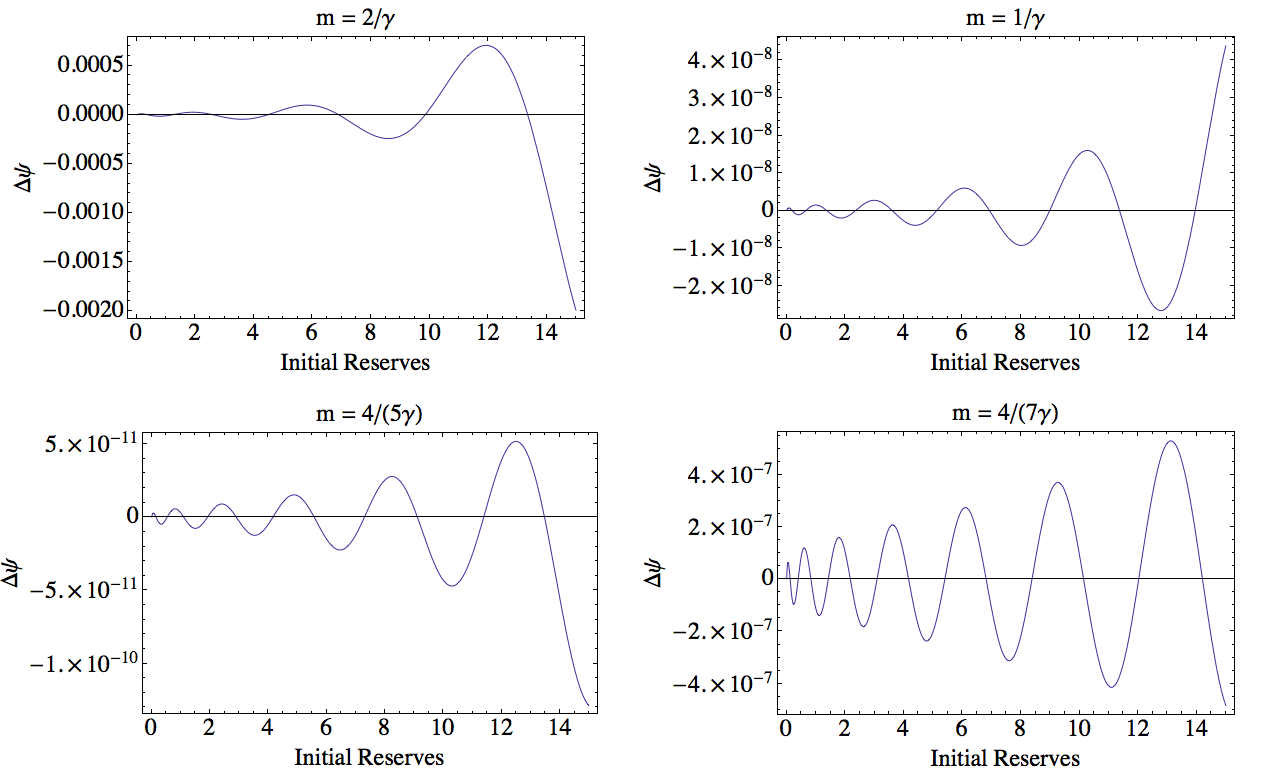
\includegraphics[width=16cm]{Chapitre4/GraphGamma2-1CasecomparisonParametrization.png}
			\caption{Difference between exact and polynomial approximations of ruin probabilities for $\Gamma(2,1)$-distributed claim sizes using different parametrizations and an order of truncation $K=40$.}\label{Gamma2CaseDifferentParametrization}
		\end{center}
	\end{figure}
\end{center}

Figure \ref{Gamma2CaseDifferentMethods} shows the relative difference between exact and approximated ruin probabilities obtained via different numerical methods. Table \ref{RuinProbaTableGamma21} gives numerical values of the ultimate ruin probability computed via the different methods. 
\begin{center}
	\begin{figure}[!h]
		\begin{center}
			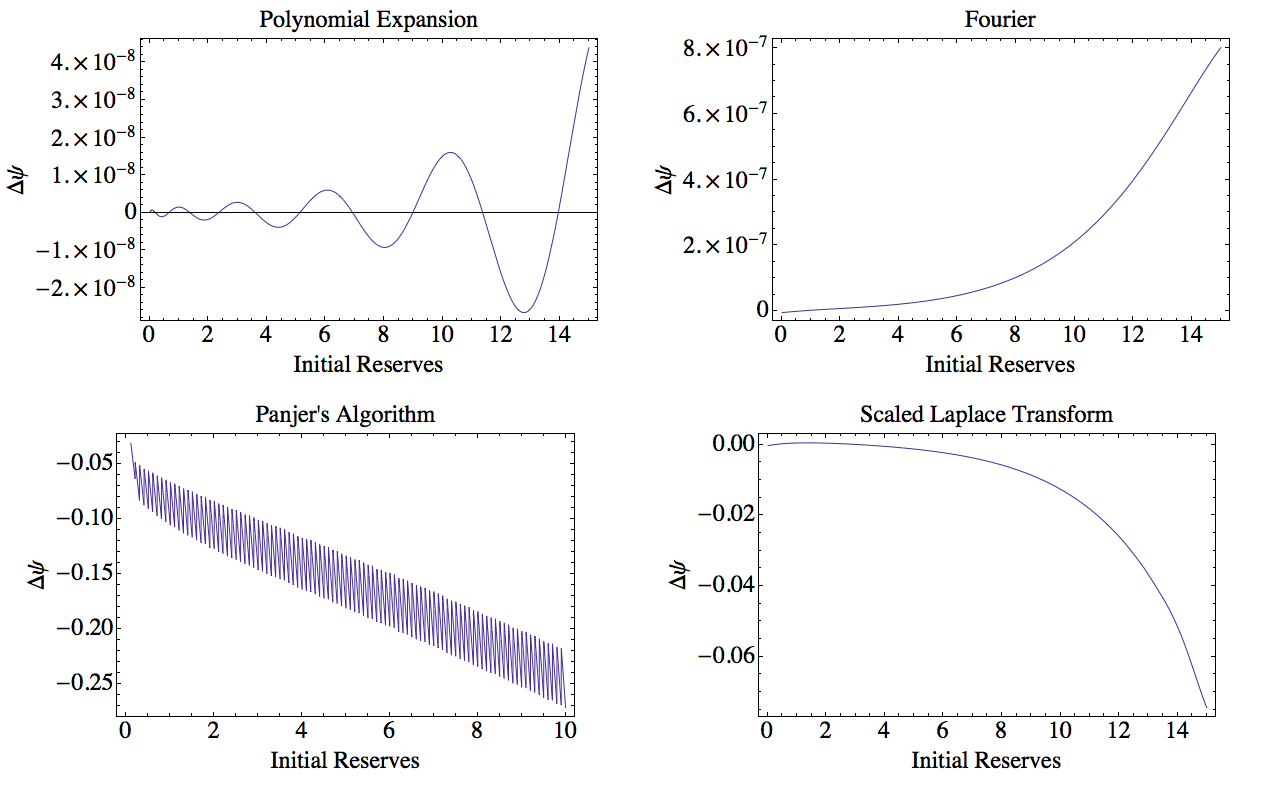
\includegraphics[width=16cm]{Chapitre4/GraphUltimateRuinProbabilityGamma2-1Case.png}
			\caption{Difference between exact and approximated ruin probabilities for $\Gamma(2,1)$-distributed claim sizes.}\label{Gamma2CaseDifferentMethods}
		\end{center}
	\end{figure}
\end{center}

\begin{table}
\begin{center}
\begin{tabular}{|c|c||c|c|c|c|}
  \hline
i&$u_{i}$&Exact&Polynomial &Fourier& Scaled Laplace\\
   && &Expansion& transform inversion &transform inversion \\
\hline
  \hline
40& 0.295528 & 0.363928 & 0.363928 & 0.363928 & 0.363907 \\
80& 0.633837 & 0.322916 & 0.322916 & 0.322916 & 0.322815 \\
120& 1.01723 & 0.279149 & 0.279149 & 0.279149 & 0.279022 \\
 160&1.45959 & 0.233859 & 0.233859 & 0.233859 & 0.233746 \\
200& 1.98243 & 0.188205 & 0.188205 & 0.188205 & 0.188129 \\
240& 2.62167 & 0.143304 & 0.143304 & 0.143304 & 0.143275 \\
280& 3.44446 & 0.100282 & 0.100282 & 0.100282 & 0.100299 \\
320& 4.60063 & 0.0604002 & 0.0604002 & 0.0604002 & 0.0604562 \\
360& 6.56208 & 0.0254366 & 0.0254366 & 0.0254366 & 0.0255143 \\
400& 17.26 & 0.000225548 & 0.000225548 & 0.000225548 & 0.000258617 \\
  \hline
\end{tabular} 
\caption{Probabilities of ultimate ruin approximated via the Fourier series method, the polynomial expansion and the scaled Laplace transform inversion when the claim amounts are $\Gamma(2,1)$-distributed.}\label{RuinProbaTableGamma21}
\end{center}
\end{table}
The polynomial expansion gives the best results, even better than the Fourier series based method in this case. In the second case, we assume that the claim amounts are $\Gamma(3,1)$-distributed and the premium are collected at $p=3.6$. This setting implies a smaller safety loading than in the previous case and therefore greater ruin probabilities with respect to a given initial reserve. In this case, the exact probability of ultimate ruin is given by
\begin{eqnarray*}\label{ExactRuinProbabilityGamma31}
\psi(u)&=& 0.861024e^{-0.0859017 u}-0.0196231e^{-1.31816
   u} \sin (0.450173 u)\\
&-&0.0276908e^{-1.31816 u} \cos (0.450173 u)
\end{eqnarray*}
The adjustment coefficient is $\gamma \approx 0.086$.\\

Figure \ref{Gamma3CaseDifferentMethods} displays the difference between exact and approximated ruin probabilities. We set $m=1/\gamma$ and $K=40$ for the polynomial expansion and $\{a=400,b=1.055\}$ for the scaled Laplace transform technique. Because we need to compute ruin probabilities for large initial reserves, we had to set $h=1$ in order to get an acceptable computational time using Panjer\rq{}s algorithm. The Fourier series based method performs better than the the other method in this case. Polynomial expansion and scaled Laplace transform give close results. The performance of the polynomial expansion are influenced by the settings of the ruin model. We need an higher order of truncation to get the same results as in the previous example.

\begin{center}
	\begin{figure}[!h]
		\begin{center}
			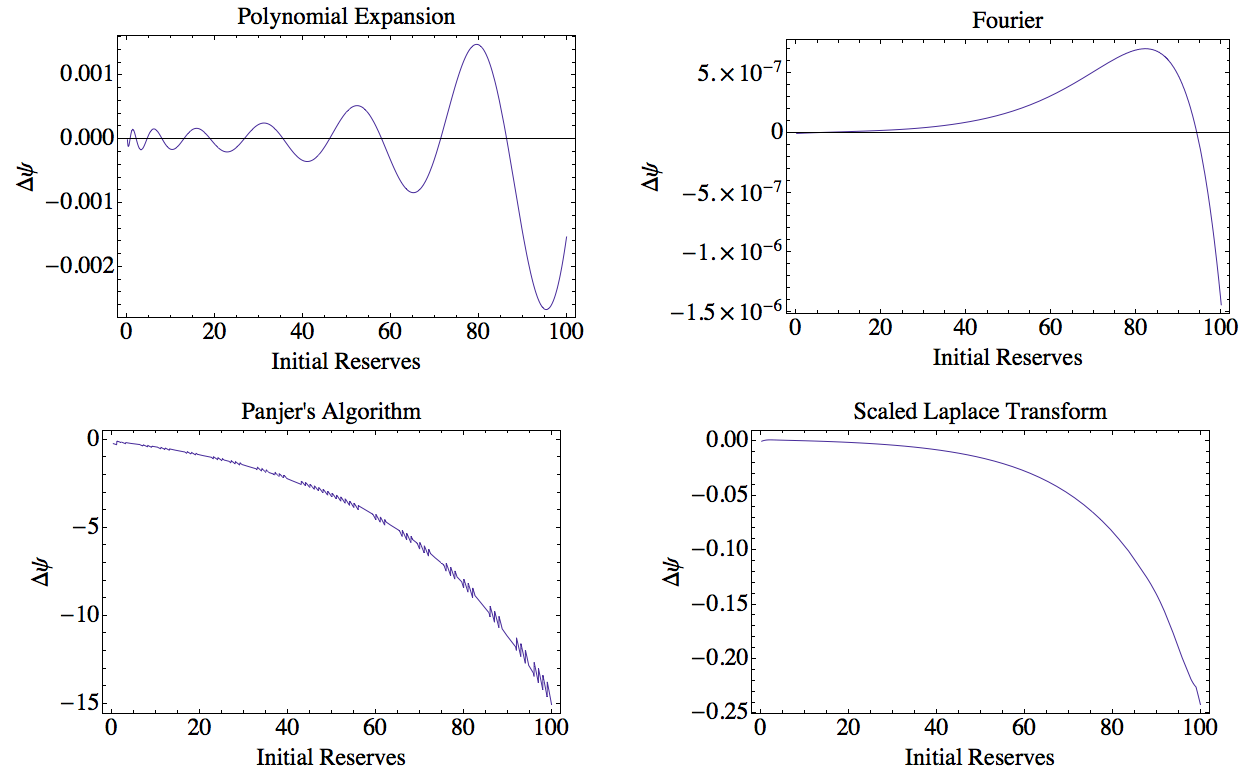
\includegraphics[width=16cm]{Chapitre4/GraphUltimateRuinProbabilityGamma3-1Case.png}
			\caption{Difference between exact and approximated ruin probabilities for $\Gamma(3,1)$-distributed claim sizes.}\label{Gamma3CaseDifferentMethods}
		\end{center}
	\end{figure}
\end{center}
\begin{table}
\begin{center}
\begin{tabular}{|c|c||c|c|c|c|}
  \hline
i&$u_{i}$&Exact&Polynomial &Fourier& Scaled Laplace\\
   && &Expansion& transform inversion &transform inversion \\
\hline
  \hline
  40 & 1.91605 & 0.727722 & 0.7277 & 0.727722 & 0.726683 \\
 80 & 4.10946 & 0.60488 & 0.604914 & 0.60488 & 0.604143 \\
 120 & 6.59516 & 0.488625 & 0.488556 & 0.488625 & 0.488154 \\
 160 & 9.46321 & 0.381922 & 0.381976 & 0.381922 & 0.381667 \\
 200 & 12.853 & 0.285439 & 0.285436 & 0.285439 & 0.285365 \\
 240 & 16.9975 & 0.199938 & 0.19991 & 0.199938 & 0.200009 \\
 280 & 22.332 & 0.126439 & 0.126464 & 0.126439 & 0.126612 \\
 320 & 29.828 & 0.0664098 & 0.0663945 & 0.0664098 & 0.0666329 \\
 360 & 42.545 & 0.0222743 & 0.0222812 & 0.0222743 & 0.0224793 \\
 400 & 111.905 & 0.0000575741 & 0.0000572446 & 0.0000575747 & 0.0000823883 \\
  \hline
\end{tabular} 
\caption{Probabilities of ultimate ruin approximated via the Fourier series method, the polynomial expansion and the scaled Laplace transform inversion when the claim amounts are $\Gamma(3,1)$-distributed.}\label{RuinProbaTableGamma31}
\end{center}
\end{table}

Our method enables us to approximate ruin probabilities in cases that are relevant for applications but where no formulas are currently available. In this last example, we suppose that the claim sizes are uniformly distributed between $0$ and $100$ and the premium are collected at $p=80$. The adjustment coefficient is $\gamma\approx0.013$. As the Fourier series based method did a good job in the previous cases, we take ruin probabilities approximated via the Fourier series technique as benchmark to assess the accuracy of the polynomial expansion. We set $K=40$ and $m=1/\gamma$ for the polynomial  expansion and $\{\alpha=200,b=1,0045\}$ for the scaled Laplace transform inversion.\\

Figure \ref{UniformCase} displays the relative difference between ruin probabilies approximated the polynomial expansion and the scaled Laplace transform inversion technique with respect to the approximation derived from the numerical inversion of the Fourier transform. Table \ref{RuinProbaTableUniform} gives approximated ruin probabilities for some initial reserves obtained via the Fourier transform inversion, the polynomial expansion, and the scaled Laplace transform inversion.
\begin{center}
	\begin{figure}[!h]
			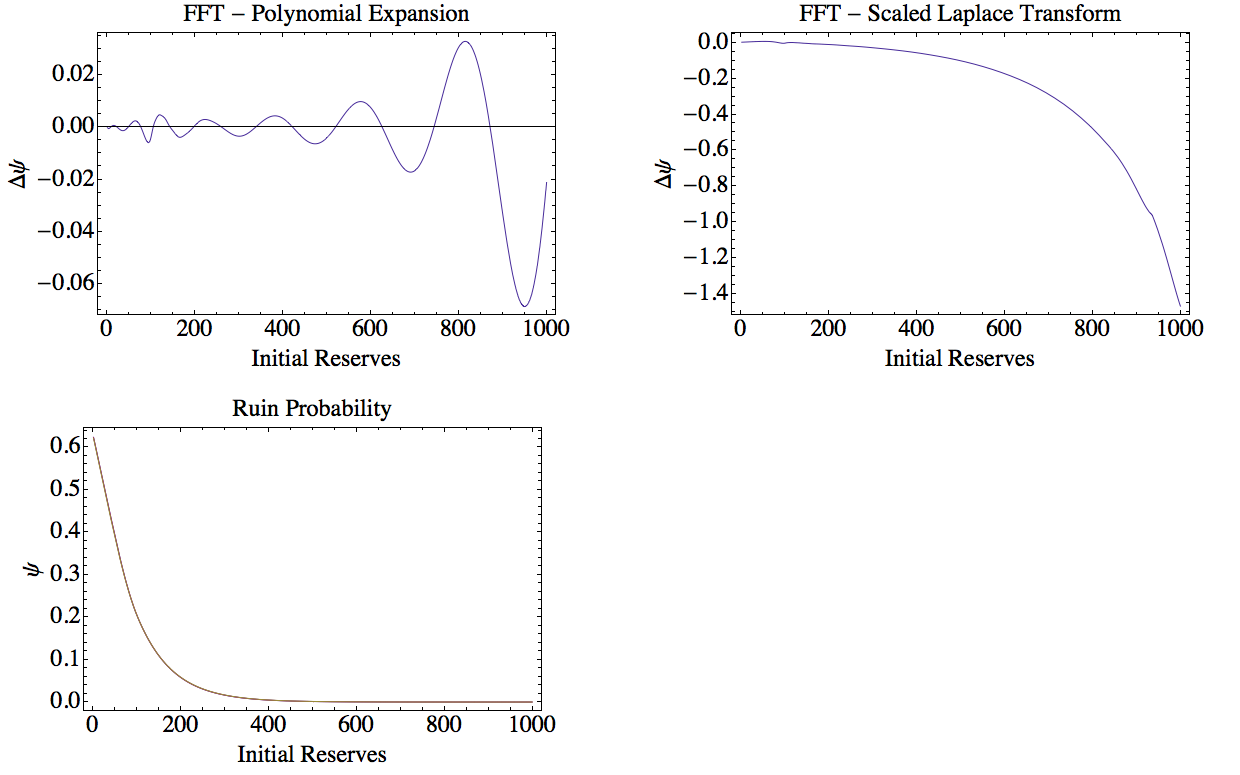
\includegraphics[width=16cm]{Chapitre4/GraphUltimateRuinProbabilityUniformCase.png}
			\caption[Relative error and ruin probabilities for $U\left(0,100\right)$-distributed claim sizes ]{(Top left) Difference between the Fourier series technique based and the polynomial approximation of the ultimate ruin probability for $U\left[0,100\right]$-distributed claim sizes. (Top right) Difference between the Fourier series technique and the scaled Laplace transform inversion approximation of the ultimate ruin probability for $U\left[0,100\right]$-distributed claim sizes. (Bottom left) Probabilities of ultimate ruin obtained via the Fourier series technique,  the polynomial expansion and the scaled Laplace transform method.}\label{UniformCase}
	\end{figure}
\end{center}

\begin{table}
\begin{center}
\begin{tabular}{|c||c|c|c|c|}
  \hline
  i& $u_{i}$ & Polynomial &Fourier&Scaled Laplace\\
  &  & expansion &transform inversion&transform \\
\hline
  \hline
 20 & 22.2322 & 0.518736& 0.518768 & 0.515691 \\
 40 & 48.3113 & 0.394639 & 0.394764 & 0.391591 \\
 60 & 77.8541 & 0.270484 & 0.27034 & 0.269242 \\
 80 & 111.924 & 0.173775 & 0.174403 & 0.174105 \\
 100 & 152.163 & 0.105036 & 0.10483 & 0.105196 \\
 120 & 201.311 & 0.0561043 & 0.0561651 & 0.0567006 \\
 140 & 264.47 & 0.0252093 & 0.0251985 & 0.0257021 \\
 160 & 352.957 & 0.00817819 & 0.00819723 & 0.00853082 \\
 180 & 501.969 & 0.0012417 & 0.00123727 & 0.00136279 \\
 200 & 1180.05 & $2.479493055\times10^{-7}$ &
$2.28077799077\times10^{-7}$ &
   $1.07450197444\times10^{-6}$ \\
  \hline
\end{tabular} 
\end{center}
\caption{Probabilities of ultimate ruin approximated via the Fourier series method, the polynomial expansion and the scaled Laplace transform inversion when the claim amounts are $U\left[0,100\right]$-distributed.}\label{RuinProbaTableUniform}
\end{table}
The difference between the polynomial approximation and the Fourier series approximation is small, and we see on Figure \ref{UniformCase} that the ruin probability curves overlap.  
\clearpage
\section{Conclusion}
Our method provides a very good approximation of the ruin probability when the claim sizes distribution is light-tailed. We obtained a theoretical result that ensures the validity of our expansions. As expected, the numerical results show the superiority of the Fourier series based method in term of accuracy. Nevertheless, our method provides an approximation of a simple form for the whole ruin function and allows reinjection to derive approximations of other quantities of interest in ruin theory. Another advantage is the possibility of a statistical extension that will lead to a nonparametric estimation of ruin probabilities just like the scaled Laplace transform inversion and maximum entropy methods. The great results in terms of accuracy are promising and it will be interesting to consider statistical application. It is also worth noting that this method can be easily adapted to a multivariate problem. The inversion of a bivariate Laplace transform will be at the center of a forthcoming paper.
\section*{Acknowledgement}
The authors would like to thank X. Guerrault for helpful discussions. The authors are also very grateful to an anonymous referee for his comments which improve greatly the quality of this paper and for the data he has provided regarding the approximation via the scaled Laplace transform inversion. This work is partially funded by the Research Chair {\it Actuariat Durable} sponsored by Milliman, and AXA research fund sponsored by AXA.

\bibliographystyle{francaissc}
\bibliography{Chapitre4/BiblioChap4}